\begin{paracol}{2}
\begin{rightcolumn*}
  \emph{July 2nd, 2004, shortly after midnight}
\end{rightcolumn*}
\begin{leftcolumn}
My emotions are gaining distinct colors, like a kind of twisted synaesthesia.  There's definitely a sense of physical location associated with each emotion, and it's not always internal.  There may also be a tactile part to this, but I have yet to experience it in any different places or with any different touches, so it may just be one continuous headache that goes latent occasionally.

An example: when pondering ****, a luminescent fuschia color that seems to be flowing in the right hemisphere of my brain; when thinking of ******* and snuggling, a warm, earthy brown with a little bit of green in a pine-needle-ish pattern about a foot and a half in front of me and slightly to the left; tiredness is off-white everywhere and blind hopelessness is bright blue wrapped around my mind.  The headache moves around, but it's mostly at the lower, back, right side of my head.  Ibuprofin works well.

This isn't what I meant when I was talking about beautiful pain.

Current mood: Bright blue with a tinge of purple, but mostly off white and hazy.
\end{leftcolumn}
\end{paracol}


\includepdf{assets/static/color/blue_flag.pdf}
\newpage

\begin{paracol}{2}
\begin{rightcolumn*}
July 3rd, 2004, shortly after midnight.
\end{rightcolumn*}
\begin{leftcolumn}
Greens covering my chest and shoulders warmly are happiness.
\vfill
\end{leftcolumn}
\end{paracol}

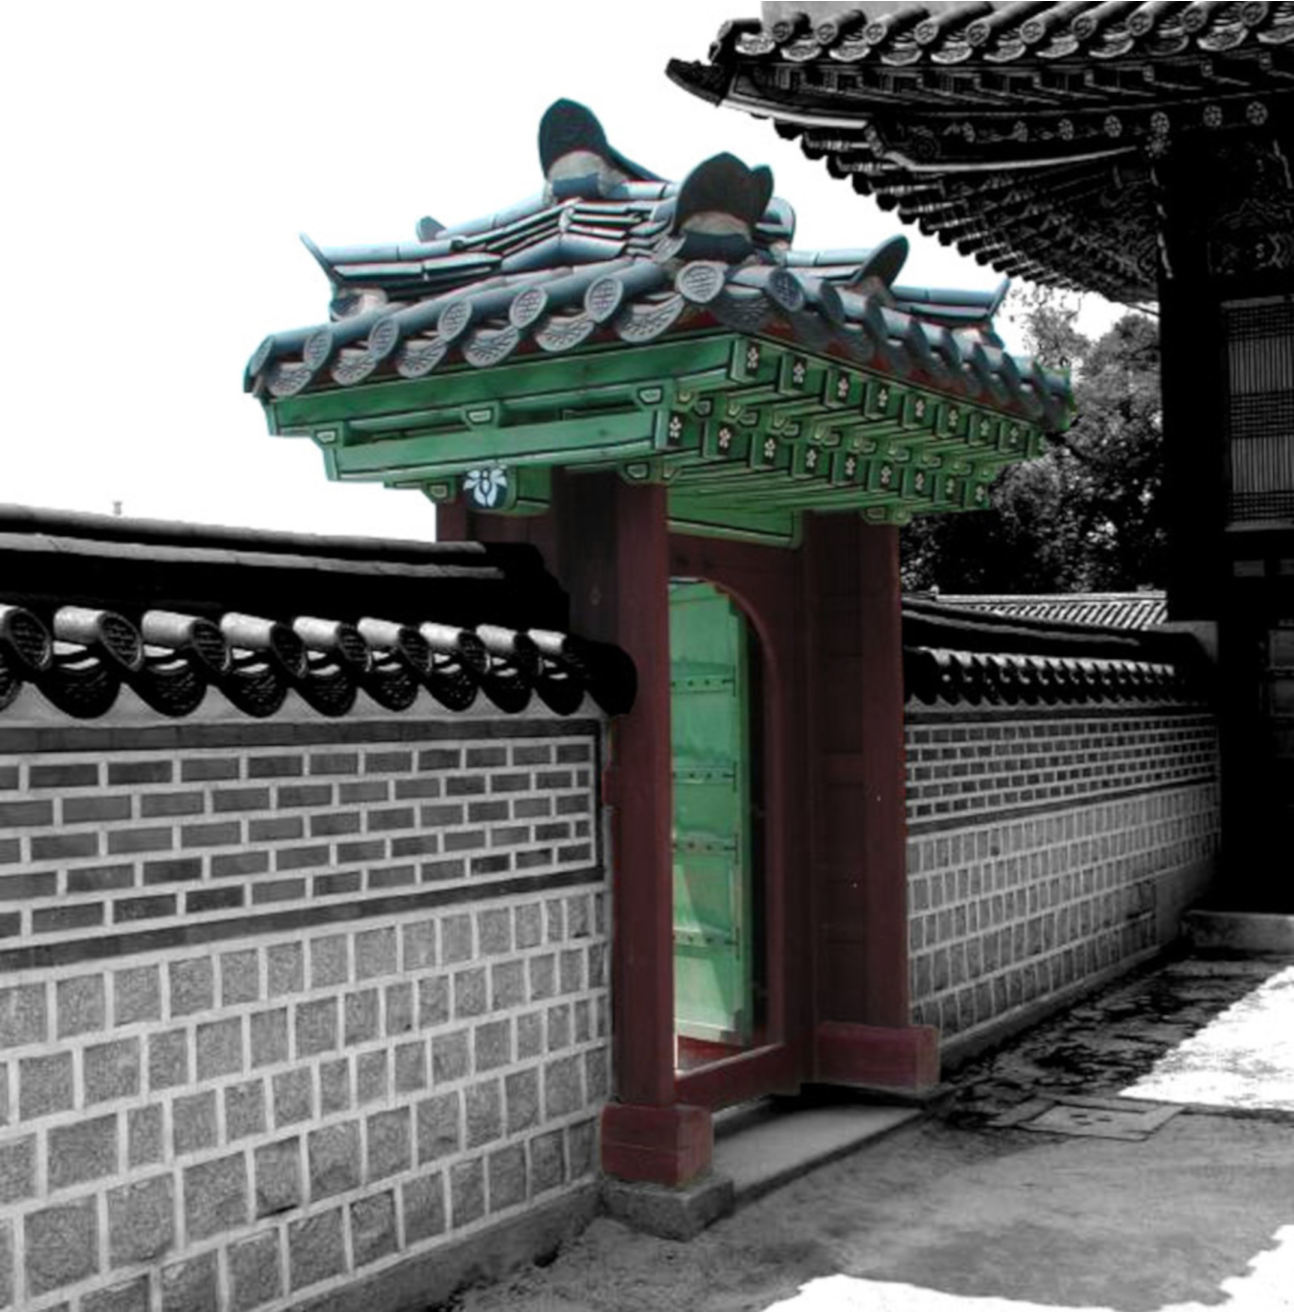
\includepdf{assets/static/color/green_door.pdf}

\begin{paracol}{2}
\begin{leftcolumn}
\begin{ally}
And that's when I showed up, yes?
\end{ally}
Yeah, later that day.

\begin{quotation}
The navy blue I've been seeing at waist level in front of me and to my left is contentment.  I'm not entirely sure that it being omnipresent is a good thing, however, considering the colors it's mixed with.  Am I really content with longing and hopelessness?  It's not out of the question, I suppose that it could just be another aspect of my personality.  But that just brings up the question of whether or not it's something I ingrained into myself through habit, something where I just kinda accepted that feeling such things is normal, okay, and what I want; or is it something I was born with, or that we're all born with?  Is it a side effect of love, expecting impossible desires and the blind hopelessness that follows the end of a four year undertaking?

\begin{ally}
Whatever, you're rambling.
\end{ally}
Guilty, conspirator.
\end{quotation}

\newpage

\begin{ally}
And these pictures?
\end{ally}
All from years later. The color thing comes and goes, like you.
\end{leftcolumn}
\begin{rightcolumn*}
\begin{flushright}
\emph{April 8, 2004}
\end{flushright}
\end{rightcolumn*}
\begin{leftcolumn}
\begin{verse}
The undersides\\
\vin \vin off gray\\
\vin of clouds\\
\vin drift\\
\vin \vin while I\\
\vin \vin \vin on the path\\
\vin \vin stand\\
\vin above\\
\vin \vin where the crow flies\\
\vin me.\\
Off\\
\vin \vin with purple\\
\vin gray, I\\
\vin \vin wandering\\
\vin ponder, should\\
\vin \vin in a perfect\\
\vin \vin \vin were there such a thing\\
\vin \vin world\\
\vin be a\\
\vin \vin though the word is plain\\
\vin color with it's own\\
\vin \vin to name\\
\vin \vin \vin as they say\\
\vin \vin creates\\
\vin word.\\
It soothes.
\end{verse}

Sometimes I'm overcome by the numinous. Sometimes it's colors, sometimes it's you, sometimes it's a silence swelling within my chest, stealing breath.

\begin{ally}
He would be riding on the subway or writing formulas on the blackboard or having a meal or (as now) sitting and talking to someone across a table, and it would envelop him like a soundless tsunami.
\end{ally}
That's a post-rock song title.

\begin{ally}
Is it wrong?
\end{ally}
\end{leftcolumn}
\end{paracol}


\includepdf{assets/static/color/orange_eyes.pdf}

\begin{paracol}{2}
  \begin{leftcolumn}
I'll take a picture, lasso a color, and desaturate everything else. Sometimes, it's fun. I do it to Falcon's eyes a lot because they're so pretty.

\begin{ally}
And sometimes it's something more.
\end{ally}
Yeah. Sometimes it's a compulsion. Sometimes a picture will latch onto me and never let me go. Sometimes I'll remove all color.
\end{leftcolumn}
\end{paracol}


% XXX Too jaggy
% 
\includepdf{assets/static/color/bw1.pdf}


\includepdf{assets/static/color/bw2.pdf}

\begin{paracol}{2}
  \begin{leftcolumn}
Sometimes I'll blow out the background because the foreground is so completely overwhelming.
\end{leftcolumn}
\end{paracol}

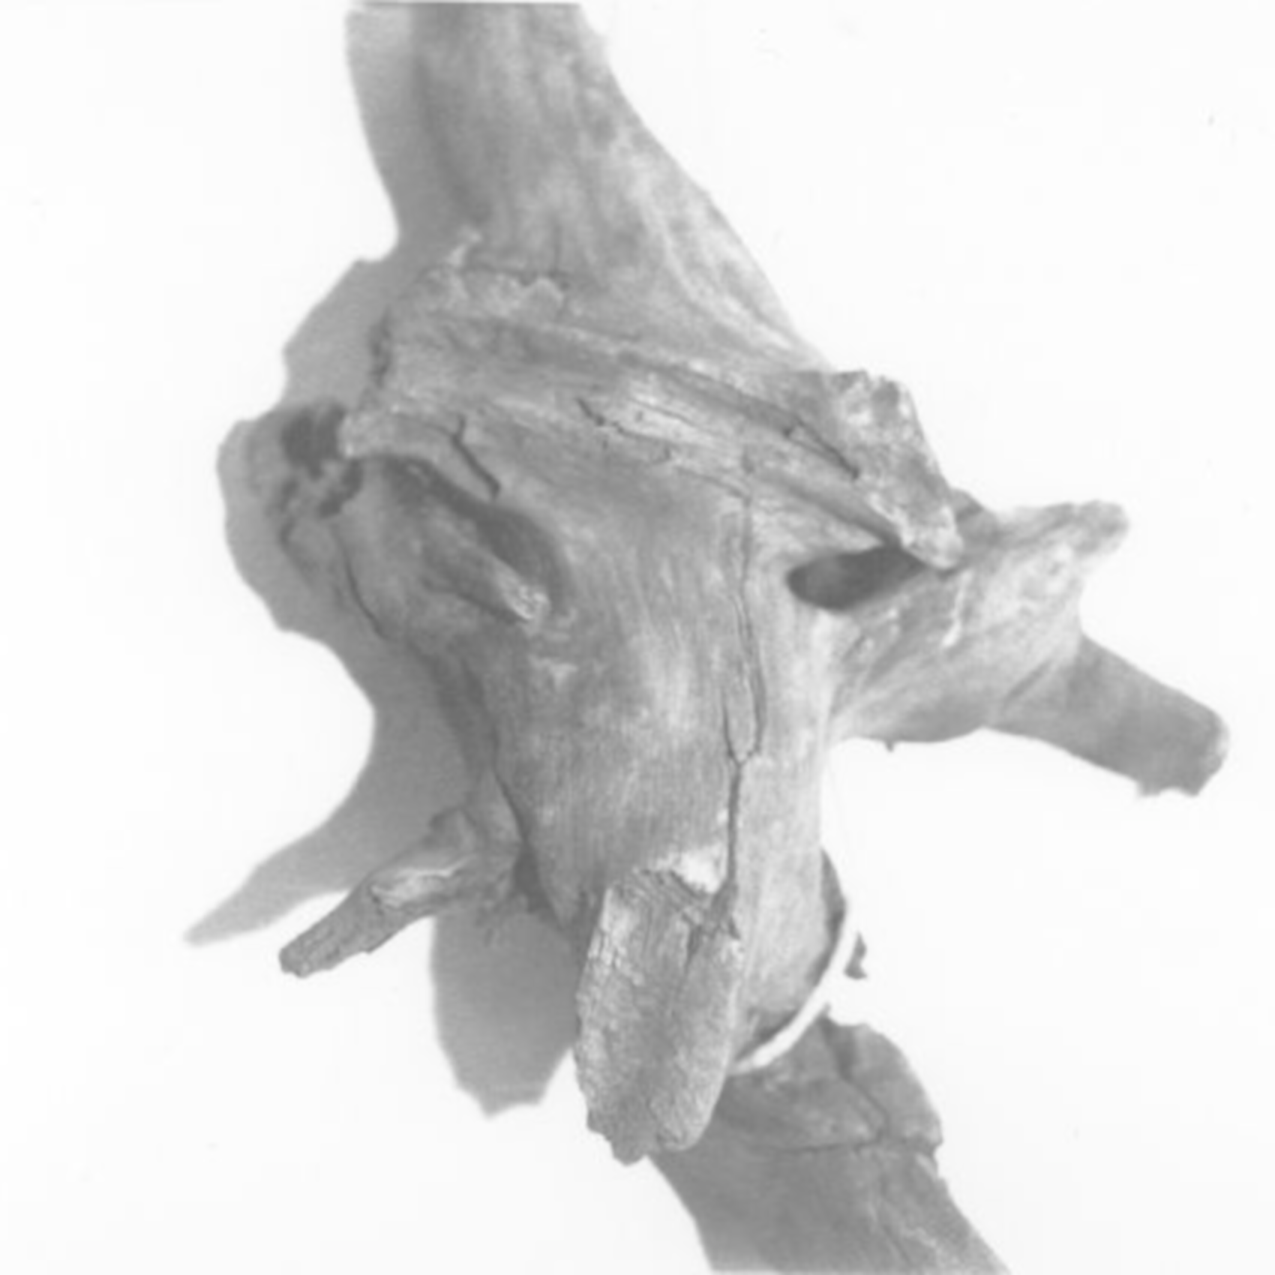
\includepdf{assets/static/color/bw3.pdf}

\null
\vfill
Sometimes I'll skew colors all in one direction.
\vfill

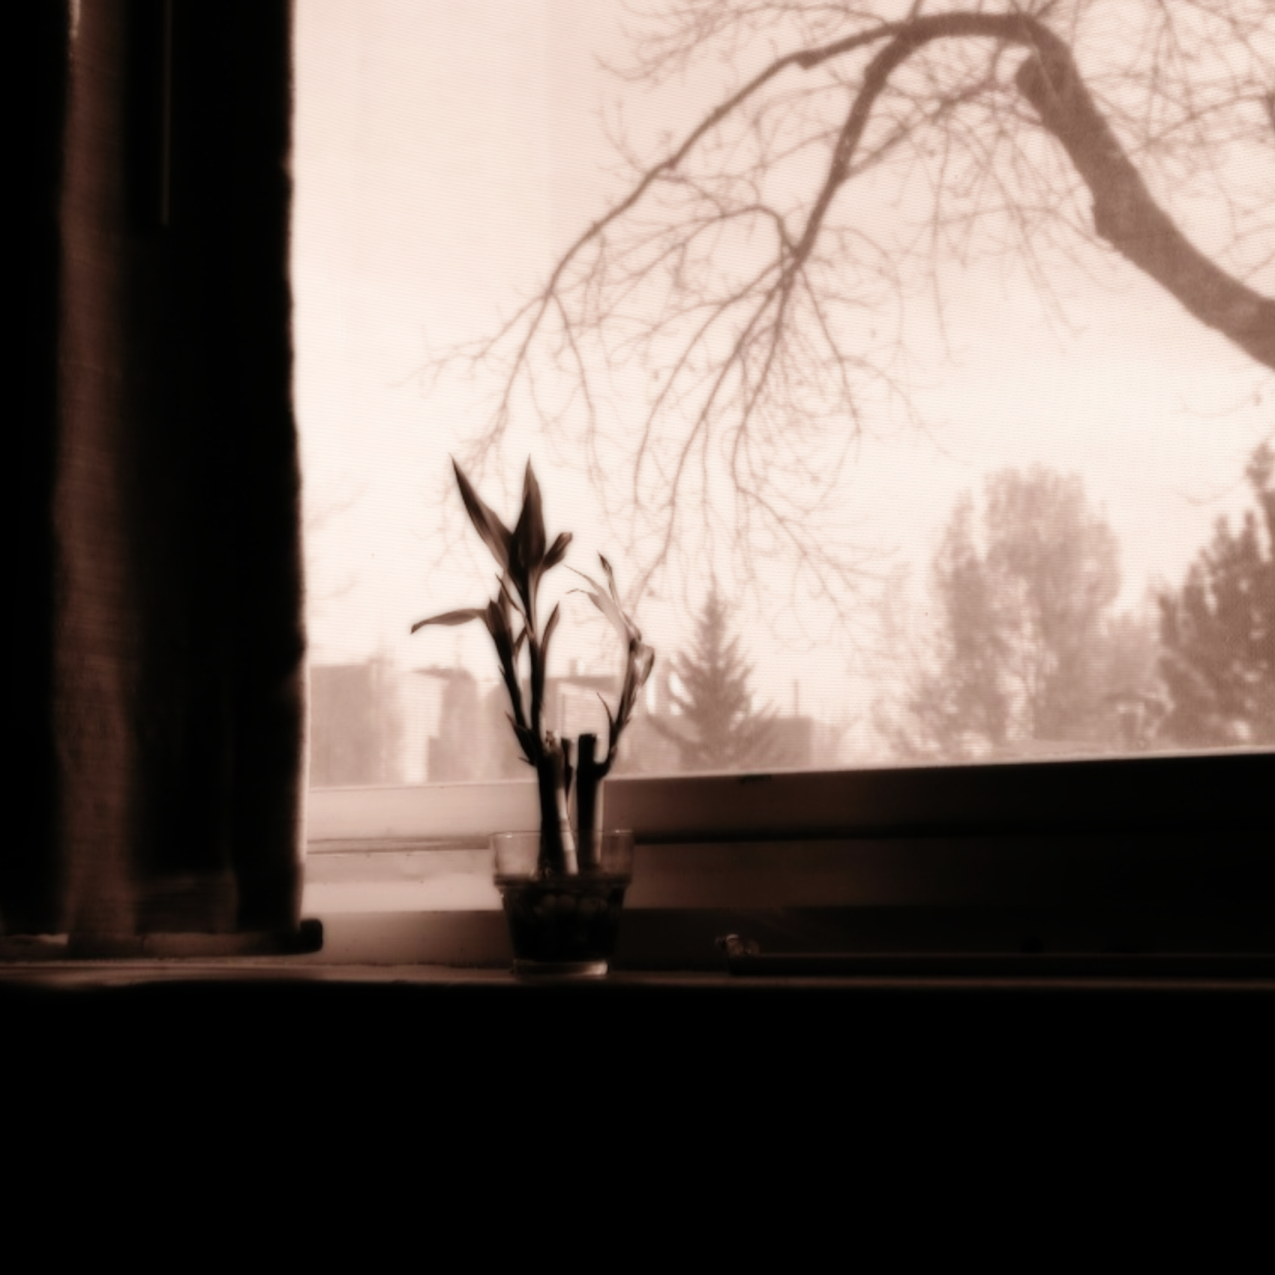
\includepdf{assets/static/color/window_view.pdf}

\vfill
\newpage

\begin{paracol}{2}
\begin{rightcolumn}
    \null
    \vfill
    \noindent
\includegraphics[width=2.5in]{assets/3.png}

    \begin{quote}
    \emph{Lines and curves, lines and curves. Beginning now.}
    \end{quote}
\end{rightcolumn}
\begin{leftcolumn}
It's not an artistic decision. Not \emph{just}, at least. It's always something more.

\begin{verse}
Inter ĝuo kaj timo\\
Estas loko de tro da signifo.\\
Apud kompreno, ekster saĝo,\\
Tamen ĝi tutampleksas.\\
Mi kompareble malgrandas\\
Kaj ĝi tro granda estas.\\
Nekomprenebla\\
Nekontestebla,\\
Senmova kaj ĉiam ŝanĝiĝema.

Between joy and fear\\
Is a place of too much meaning.\\
Next to understanding, outside wisdom,\\
It nonetheless expands.\\
I'm so small beside it\\
and it is too big.\\
Incomprehensible,\\
Incontestible,\\
Unmoving and always changing.
\end{verse}

A sigil need not just be lines and curves.

\begin{ally}
Or maybe it's just mania.
\end{ally}
It may be.
\newpage
\end{leftcolumn}
\end{paracol}
